\newcommand{\outlierFig}{
  \begin{figure}
  \centering
  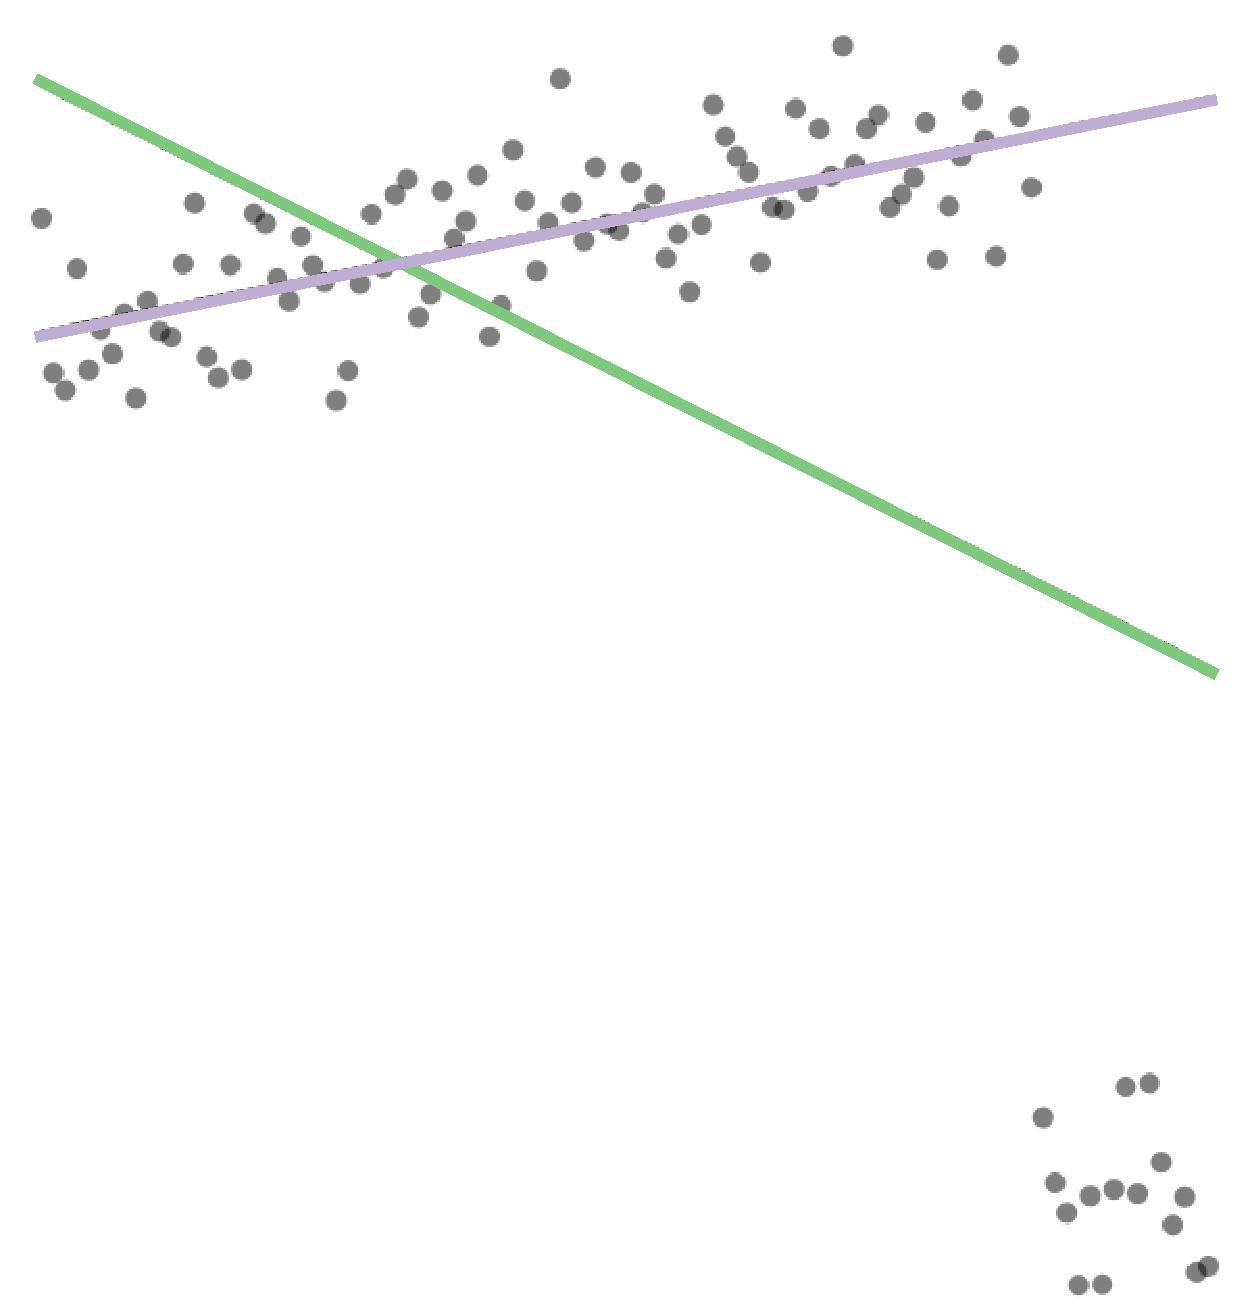
\includegraphics[width=.55\columnwidth]{figures/exp4}
  \caption{A cropped example stimulus from experiment 3. We replaced the final 15 points of this dataset with extreme values. The overlaid purple trend line represents a robust OLS fit (ignoring the outlier values), while the overlaid green line represents the fit with all points included. Participants' estimates of trend lines were universally closer to the robust than the non-robust trend; regression by eye tends to underweight outliers compared to OLS.}
  \label{fig:outlier}
  \end{figure}
}

\newcommand{\expFig}{
  \begin{figure}
  \centering
  \includegraphics[width=.65\columnwidth]{figures/exp}
  \caption{An example estimation task from our experiments. Here, the participant must adjust the amplitude of the purple trigonometric function until it best matches a particular set of bivariate data.}
  \label{fig:experiment}
  \end{figure}
}